In this section, results are presented for the
source-void-to-absorber test problem. This is a 1-D test problem
with zero incoming flux incident on the left boundary,
a constant source in a void in the left half of the
domain, and an absorber with no source in the right half of the
domain. The test problem description is given by Table
\ref{tab:source_void_to_absorber}.

%-------------------------------------------------------------------------------
\begin{table}[htb]\caption{Source-Void-to-Absorber Test Problem Summary}
\label{tab:source_void_to_absorber}
\centering
\begin{tabular}{l l}\toprule
\emph{Parameter} & \emph{Value}\\\midrule
Domain & $\domain = (0,1)$\\
Initial Conditions & $u_0(x)=0$\\
Boundary Conditions & $u(0,t)=0 \eqc \quad t>0$\\
Direction & $\di = \mathbf{e}_x$\\
Cross Section & $\sigma(x)=\left\{\begin{array}{c l}
   0,  & x < \frac{1}{2}\\
   10, & \mbox{otherwise}\end{array}\right.$\\
Source & $q(\x,t)=\left\{\begin{array}{c l}
   1,  & x < \frac{1}{2}\\
   0,  & \mbox{otherwise}\end{array}\right.$\\
Speed & $\speed=1$\\
Exact Solution & $u(x,t)=\left\{\begin{array}{l l}
   \scalarsolution_{\text{ss}}(x), & x-t<0\\
   0, & \mbox{otherwise}
   \end{array}\right.$ \\
   & $\scalarsolution_{\text{ss}}(x) =
       \left\{\begin{array}{l l}
          e^{-10(x-\frac{1}{2})}, & x\ge\frac{1}{2}\\
          1,                      & \mbox{otherwise}
       \end{array}\right.$\\
\bottomrule\end{tabular}
\end{table}
%-------------------------------------------------------------------------------

Figure \ref{fig:source_void_to_absorber}
shows the results for this problem using SSPRK time discretization,
a CFL of 0.5, and 32 cells.
Entropy residual and jump coefficients $\entropyresidualcoef$ and
$\entropyjumpcoef$ are both 1.
Table \ref{tab:source_void_to_absorber_run_parameters} summarizes the
run parameters to generate the results in this section.
Figure \ref{fig:source_void_to_absorber_fine} shows results
for a finer mesh (256 cells) that illustrates the shortcomings of Galerkin-FCT
vs. EV-FCT: Galerkin-FCT does not necessarily converge to the
entropy solution.

%-------------------------------------------------------------------------------
\begin{table}[ht]\caption{Source-Void-to-Absorber Test Problem Run Parameters}
\label{tab:source_void_to_absorber_run_parameters}
\centering
\begin{tabular}{l l}\toprule
\emph{Parameter} & \emph{Value}\\\midrule
Number of Cells & $N_{cell} = 32, 256$\\
End Time & $t = 1$\\
CFL Number & $\nu = 0.5$\\\midrule
Entropy Function & $\entropy(u) = \frac{1}{2}u^2$\\
Entropy Residual Coefficient & $\entropyresidualcoef = 1$\\
Entropy Jump Coefficient & $\entropyjumpcoef = 1$\\
\bottomrule\end{tabular}
\end{table}
%-------------------------------------------------------------------------------
\begin{figure}[ht]
   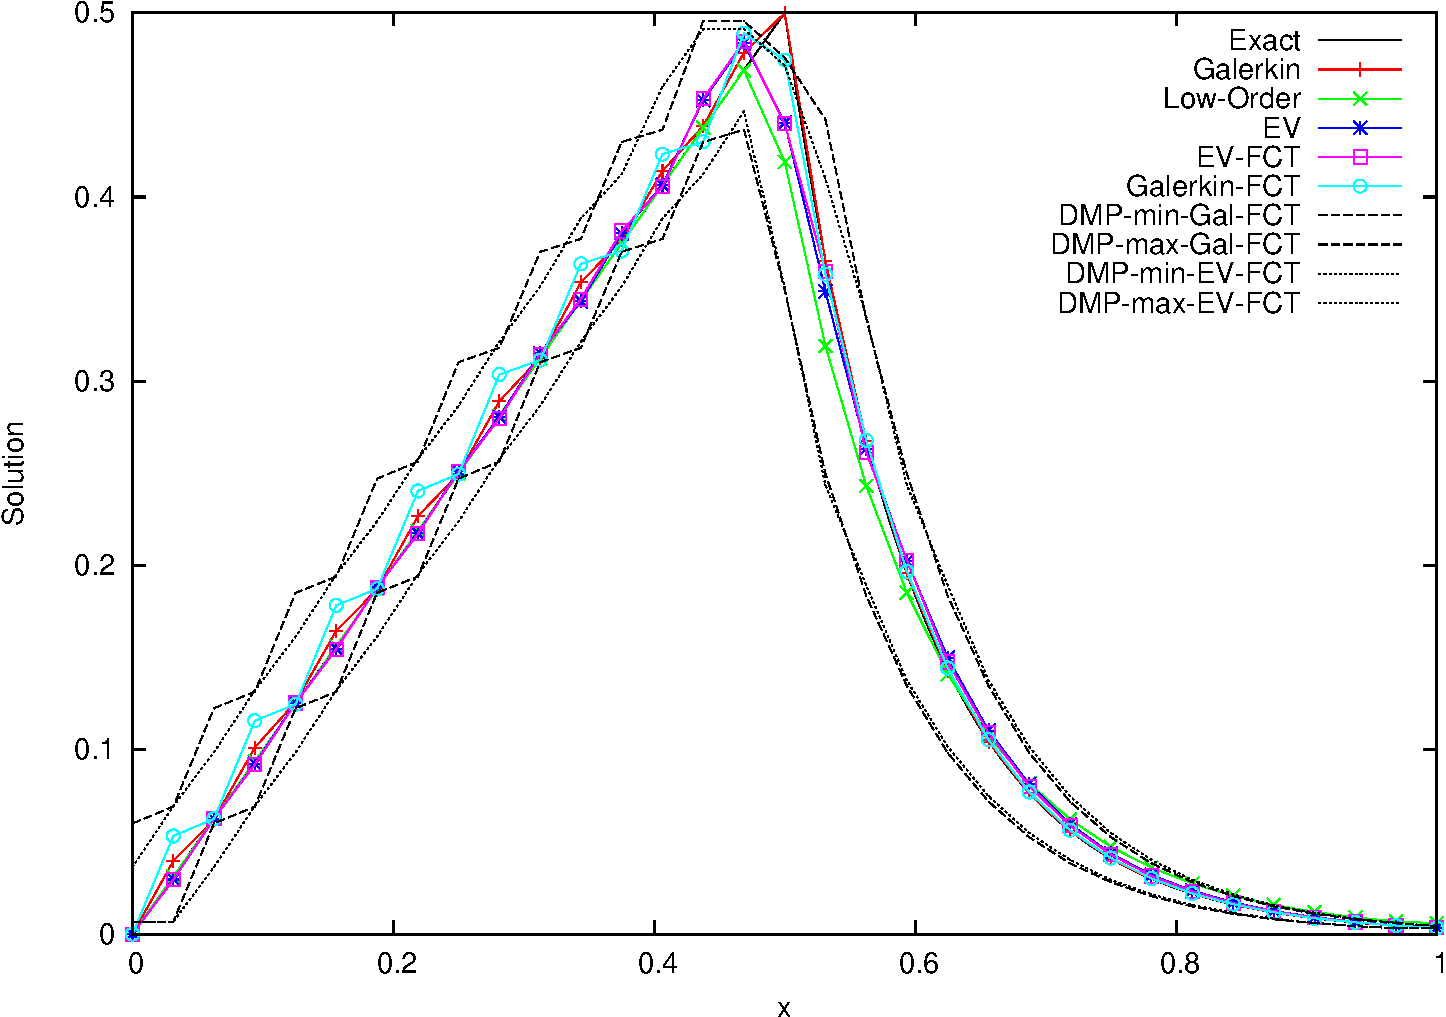
\includegraphics[width=\textwidth]
     {\contentdir/results/transport/source_void_to_absorber/coarse.pdf}
   \caption{Comparison of Solutions for the Source-Void-to-Absorber Problem
     Using SSPRK33 with 32 Cells}
   \label{fig:source_void_to_absorber}
\end{figure}
%-------------------------------------------------------------------------------
\begin{figure}[ht]
   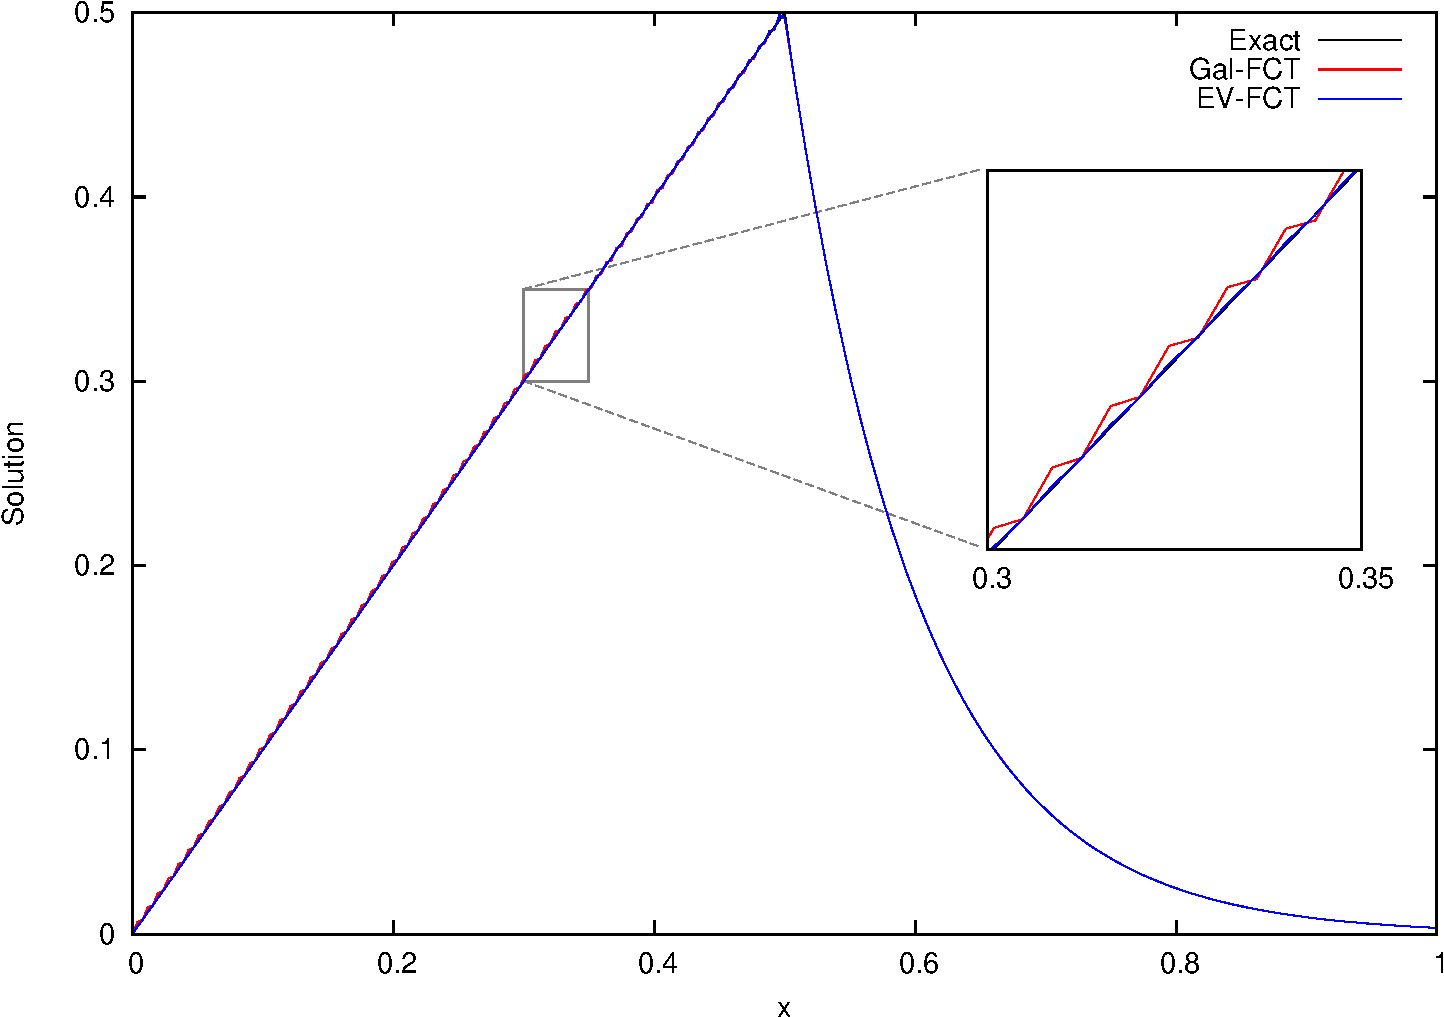
\includegraphics[width=\textwidth]
     {\contentdir/results/transport/source_void_to_absorber/fine.pdf}
   \caption{Comparison of Solutions for the Source-Void-to-Absorber Problem
     Using SSPRK33 with 256 Cells}
   \label{fig:source_void_to_absorber_fine}
\end{figure}
%-------------------------------------------------------------------------------

The steady-state results for this test problem revealed some significant
FCT issues regarding the antidiffusion from Dirichlet nodes.
When Dirichlet boundary conditions are strongly imposed, solution
bounds do not apply, and it becomes unclear how to limit antidiffusion
fluxes from these nodes. Consider symmetric limiters, i.e., those such that
$L\ij=L\ji$, such as Zalesak's limiter, for which
\begin{equation}
  L\ij = \left\{\begin{array}{c c}
    \min(L_i^+,L_j^-) & P\ij > 0\\
    \min(L_i^-,L_j^+) & P\ij < 0\\
  \end{array}\right. \eqp
\end{equation}
Suppose $i$ corresponds to a degree of freedom for which Dirichlet
boundary conditions are strongly imposed. The uncertainty
is the correct way to decide $L_i^+$ and $L_i^-$ since there
are no valid bounds from which to compute these values.
Figures \ref{fig:source_void_to_absorber_strong1} and 
\ref{fig:source_void_to_absorber_strong0} show the solutions obtained
using strongly imposed Dirichlet boundary conditions with these
values set to $L_i^+=L_i^-=1$ and $L_i^+=L_i^-=0$, respectively.
When $L_i^+=L_i^-=1$, the correction flux from the Dirichlet
DoF $i$, which is positive, has only the upper bound for $j$
to consider. The upper bound for $j$, which is inflated above the
analytical solution due to the source, does not restrict this
antidiffusion flux, and thus it is accepted fully to the unphysical
value. Due to the implicitness of the solution bounds, the lower solution
bound for $j$ is computed from this unphysical value and excludes the
possibility of antidiffusion back to the analytical solution. This
process continues with all of the other degrees of freedom.
When instead, $L_i^+=L_i^-=0$, the solution does not lie above
the analytical solution in the source region, but significant peak
clipping appears at the interface between the source and absorber
regions. It should be noted that there are combinations of limiting
coefficient values, each in the range $(0,1)$, that produce a more
accurate solution to this problem (without the peak clipping
and resulting inaccuracy in the absorber region); the problem is that Zalesak's
limiter (and in general, any practical limiter) is not optimal
in the sense that it maximizes the magnitude of antidiffusive flux.
One could in principle solve an optimization problem to select
limiting coefficients that maximize the antidiffusive flux, but this
is very expensive and thus not recommended for general use.

For weakly imposed Dirichlet boundary conditions, solution bounds
still apply, so limiting coefficients may be computed without special
consideration. However, one must now consider the possibility of
inaccurate boundary values.
Figures \ref{fig:source_void_to_absorber_weak} shows the steady-state 
solutions obtained using weakly imposed Dirichlet boundary conditions.
In this case, the antidiffusion flux from the boundary gets limited
(but not fully) due to the lower solution bound of the Dirichlet node.
Because some antidiffusion was accepted here, the peak reaches
a higher value than with the $L_i^+=L_i^-=0$ case.
Finally, Figure \ref{fig:source_void_to_absorber_penalty} shows
the steady-state solution obtained with weakly imposed Dirichlet
boundary conditions and a boundary penalty (see Section \ref{sec:transport_bc}).
The FCT solution looks very similar to the case without any penalty,
but the effect on the low-order and entropy viscosity solutions is
clear.

%-------------------------------------------------------------------------------
\begin{figure}[ht]
   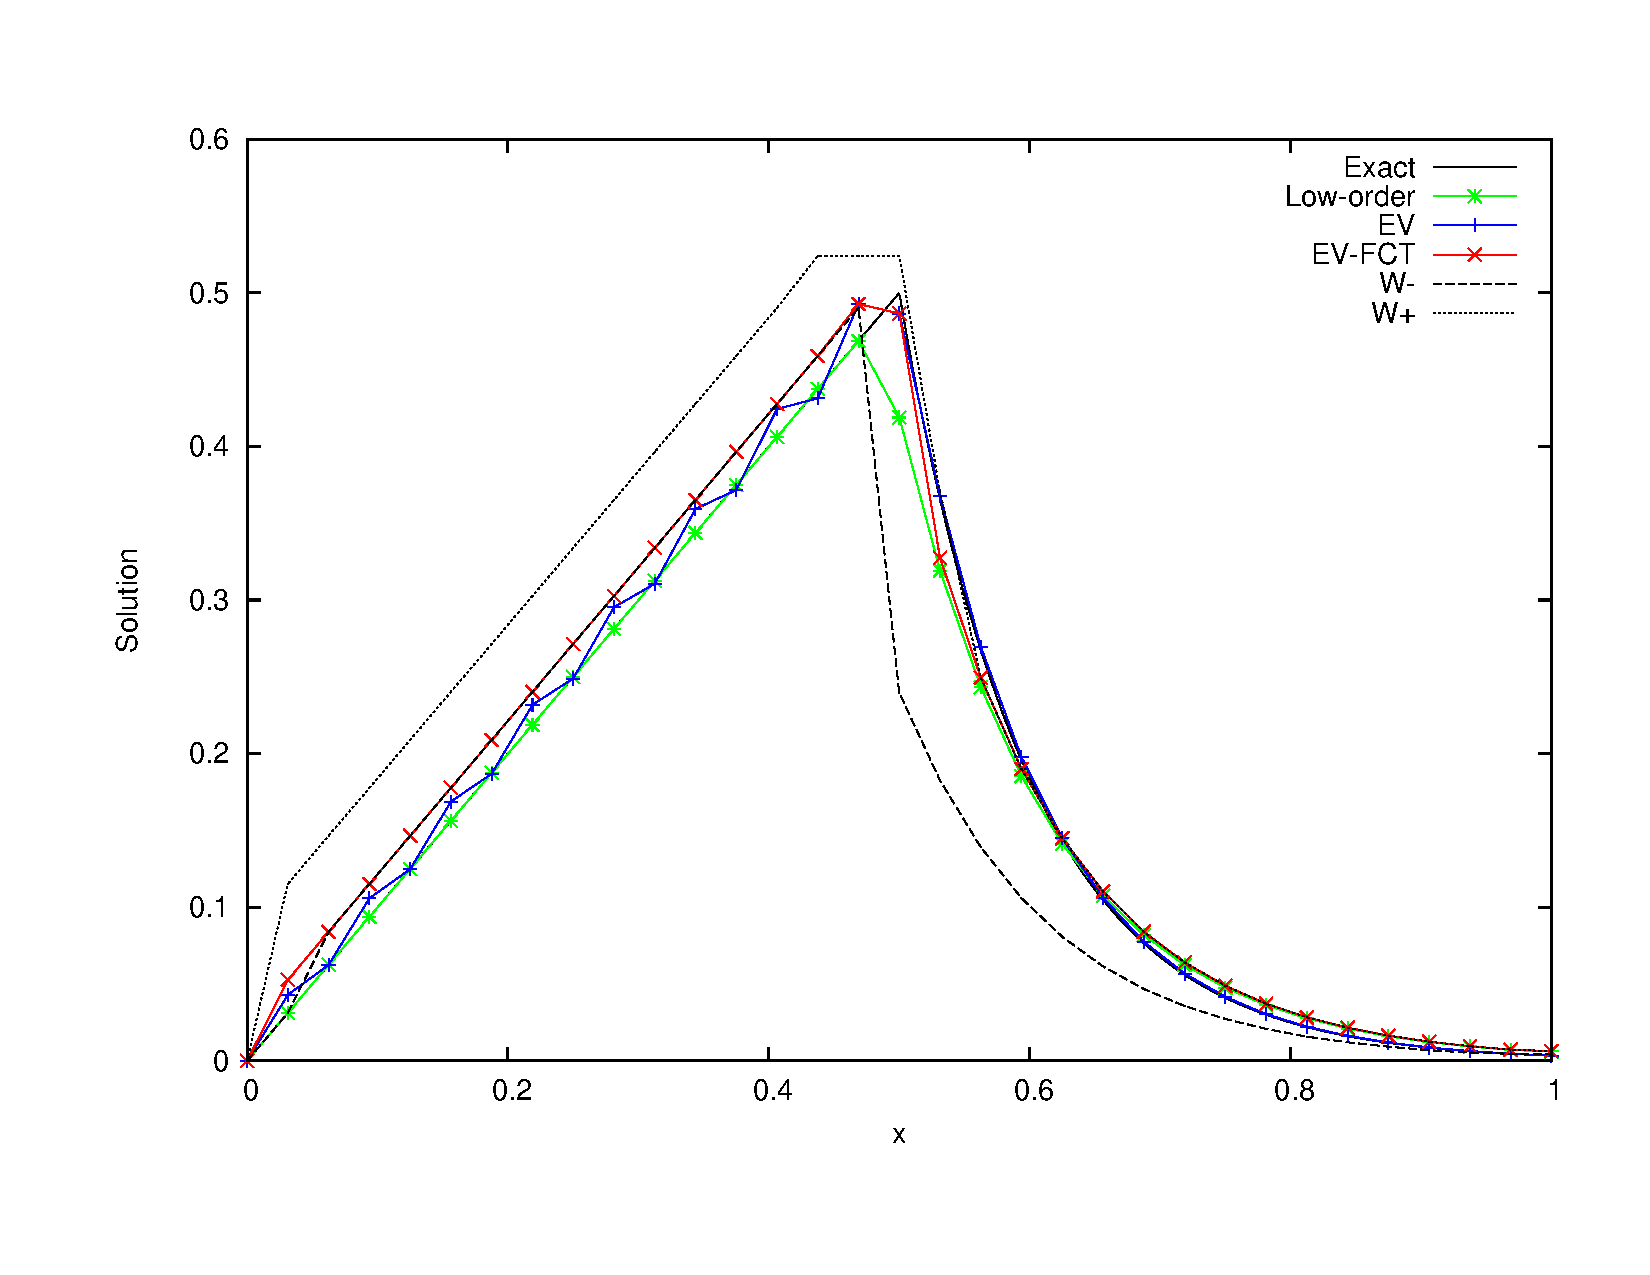
\includegraphics[width=\textwidth]
     {\contentdir/results/transport/source_void_to_absorber/images/strong1.pdf}
   \caption{Steady-State Solutions for the Source-Void-to-Absorber Problem
     with Strongly Imposed Dirichlet Boundary Conditions and $L^-=L^+=1$}
   \label{fig:source_void_to_absorber_strong1}
\end{figure}
%-------------------------------------------------------------------------------
%-------------------------------------------------------------------------------
\begin{figure}[ht]
   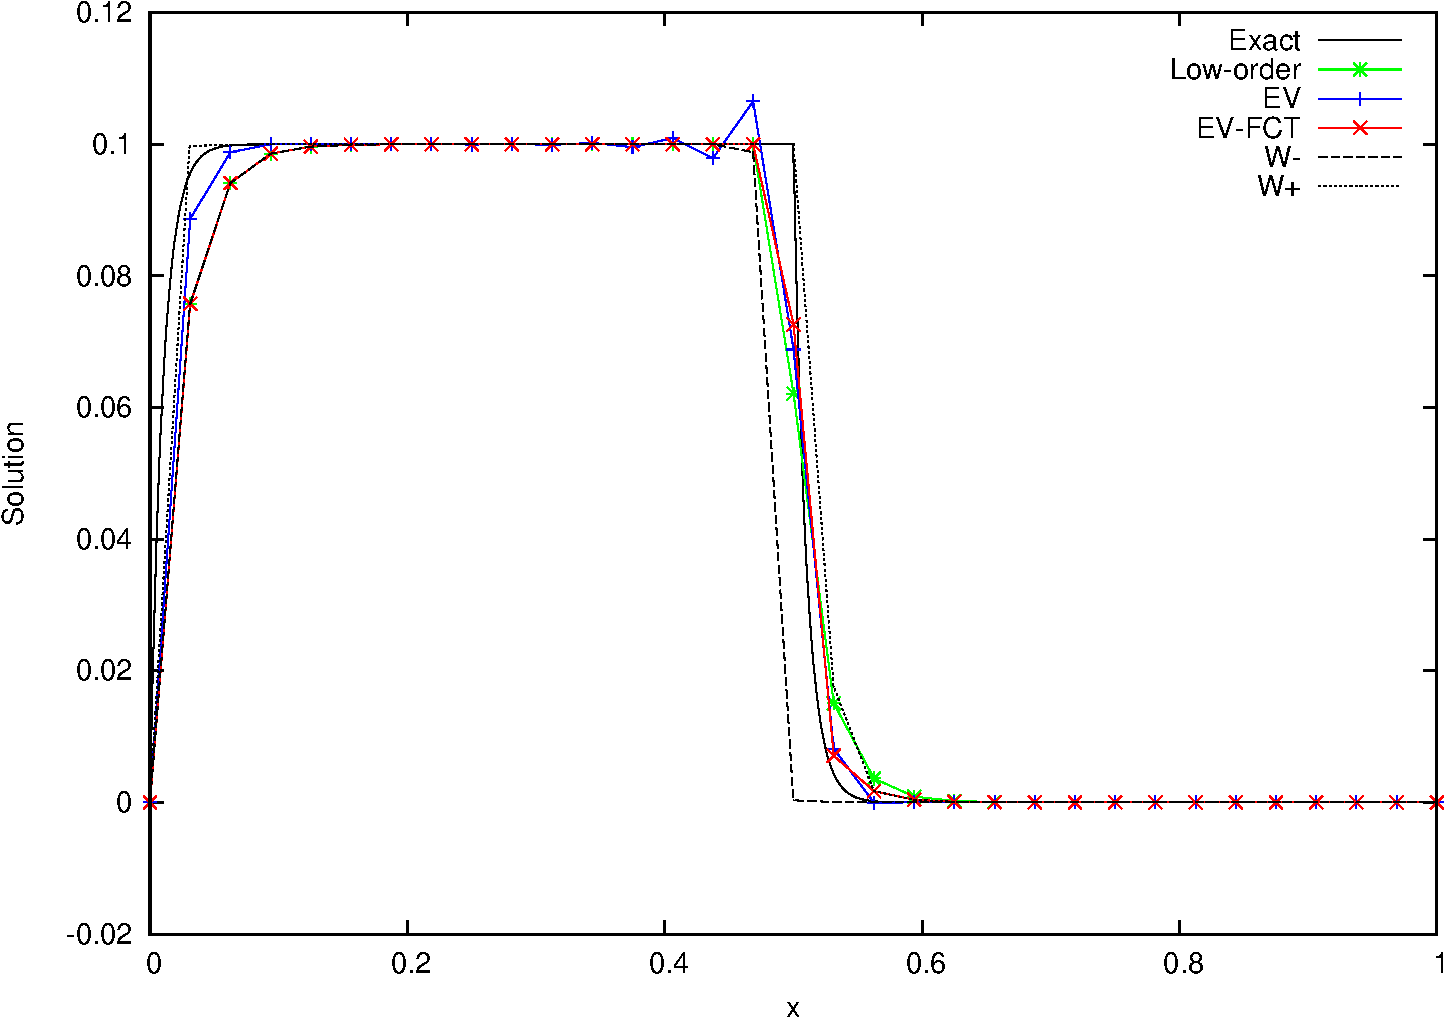
\includegraphics[width=\textwidth]
     {\contentdir/results/transport/source_void_to_absorber/images/strong0.pdf}
   \caption{Steady-State Solutions for the Source-Void-to-Absorber Problem
     with Strongly Imposed Dirichlet Boundary Conditions and $L^-=L^+=0$}
   \label{fig:source_void_to_absorber_strong0}
\end{figure}
%-------------------------------------------------------------------------------
%-------------------------------------------------------------------------------
\begin{figure}[ht]
   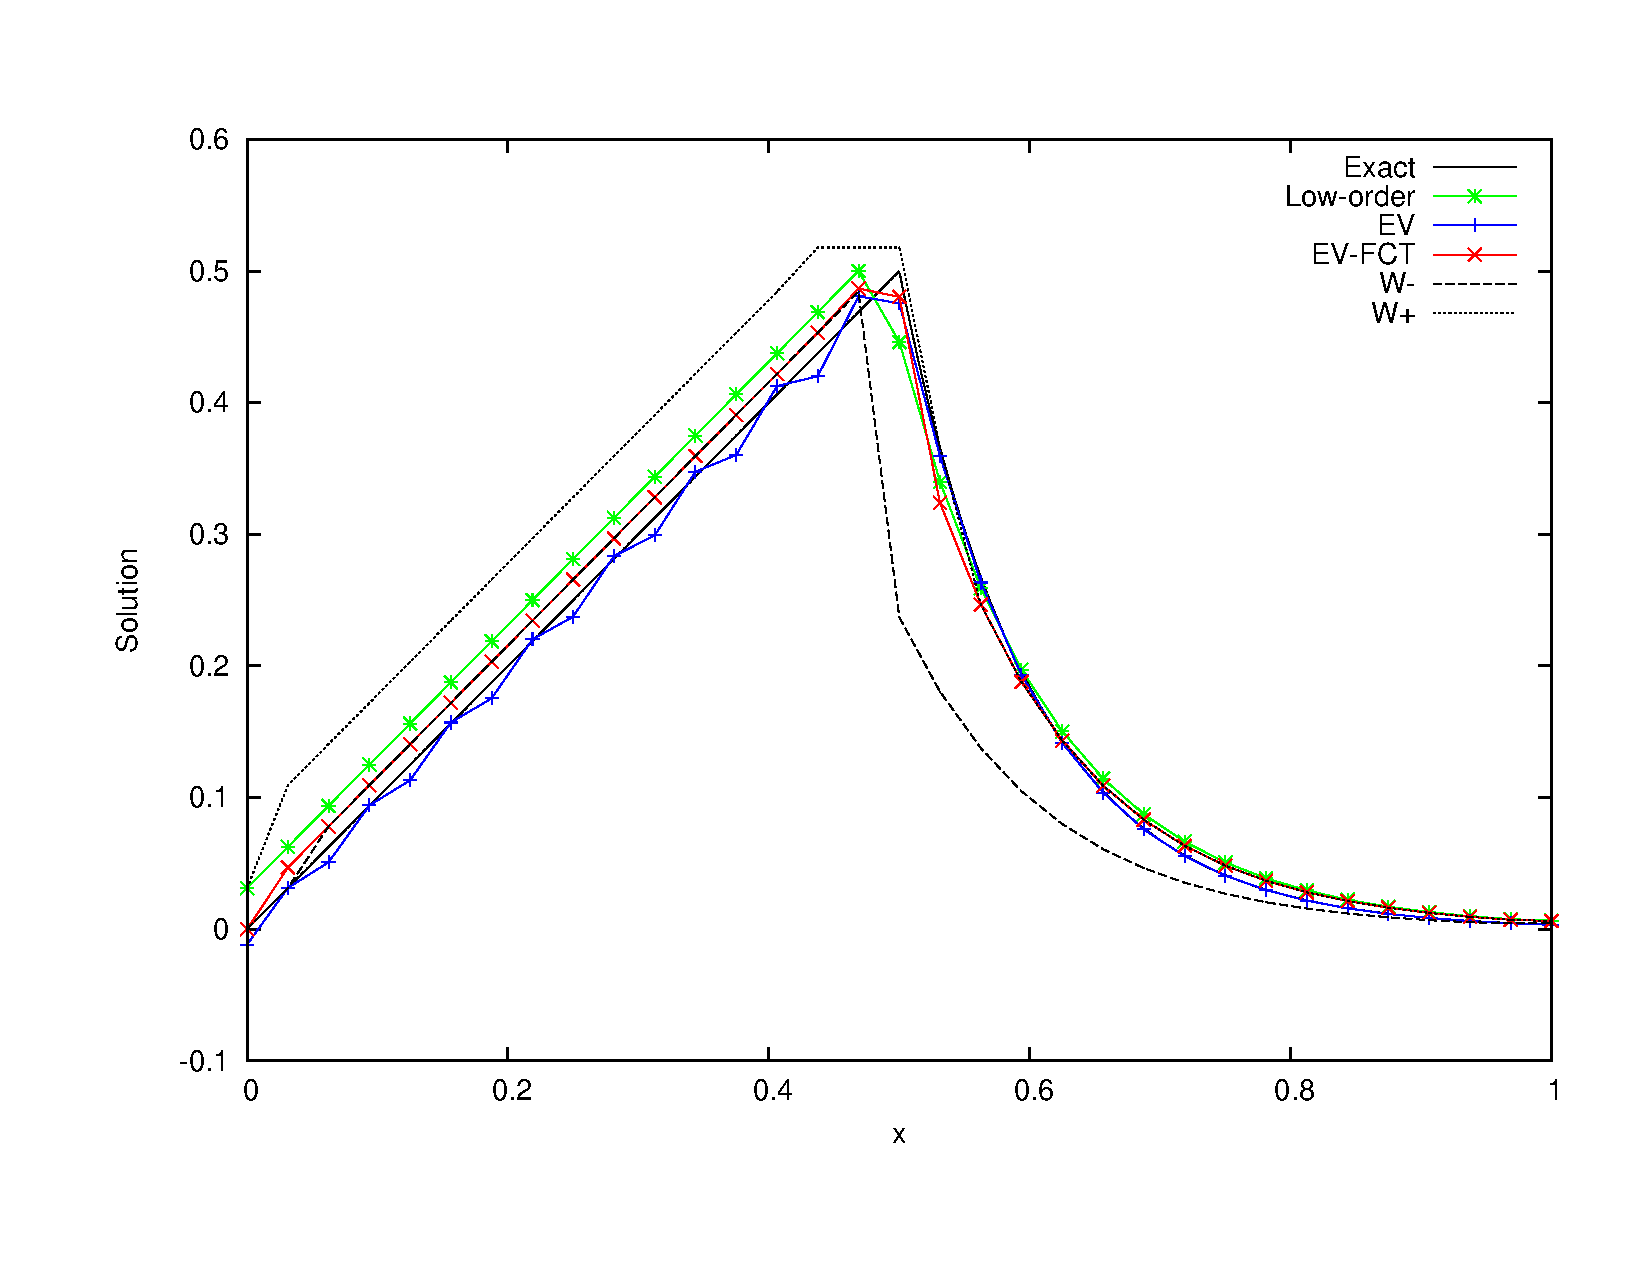
\includegraphics[width=\textwidth]
     {\contentdir/results/transport/source_void_to_absorber/images/weak.pdf}
   \caption{Steady-State Solutions for the Source-Void-to-Absorber Problem
     with Weakly Imposed Dirichlet Boundary Conditions}
   \label{fig:source_void_to_absorber_weak}
\end{figure}
%-------------------------------------------------------------------------------
%-------------------------------------------------------------------------------
\begin{figure}[ht]
   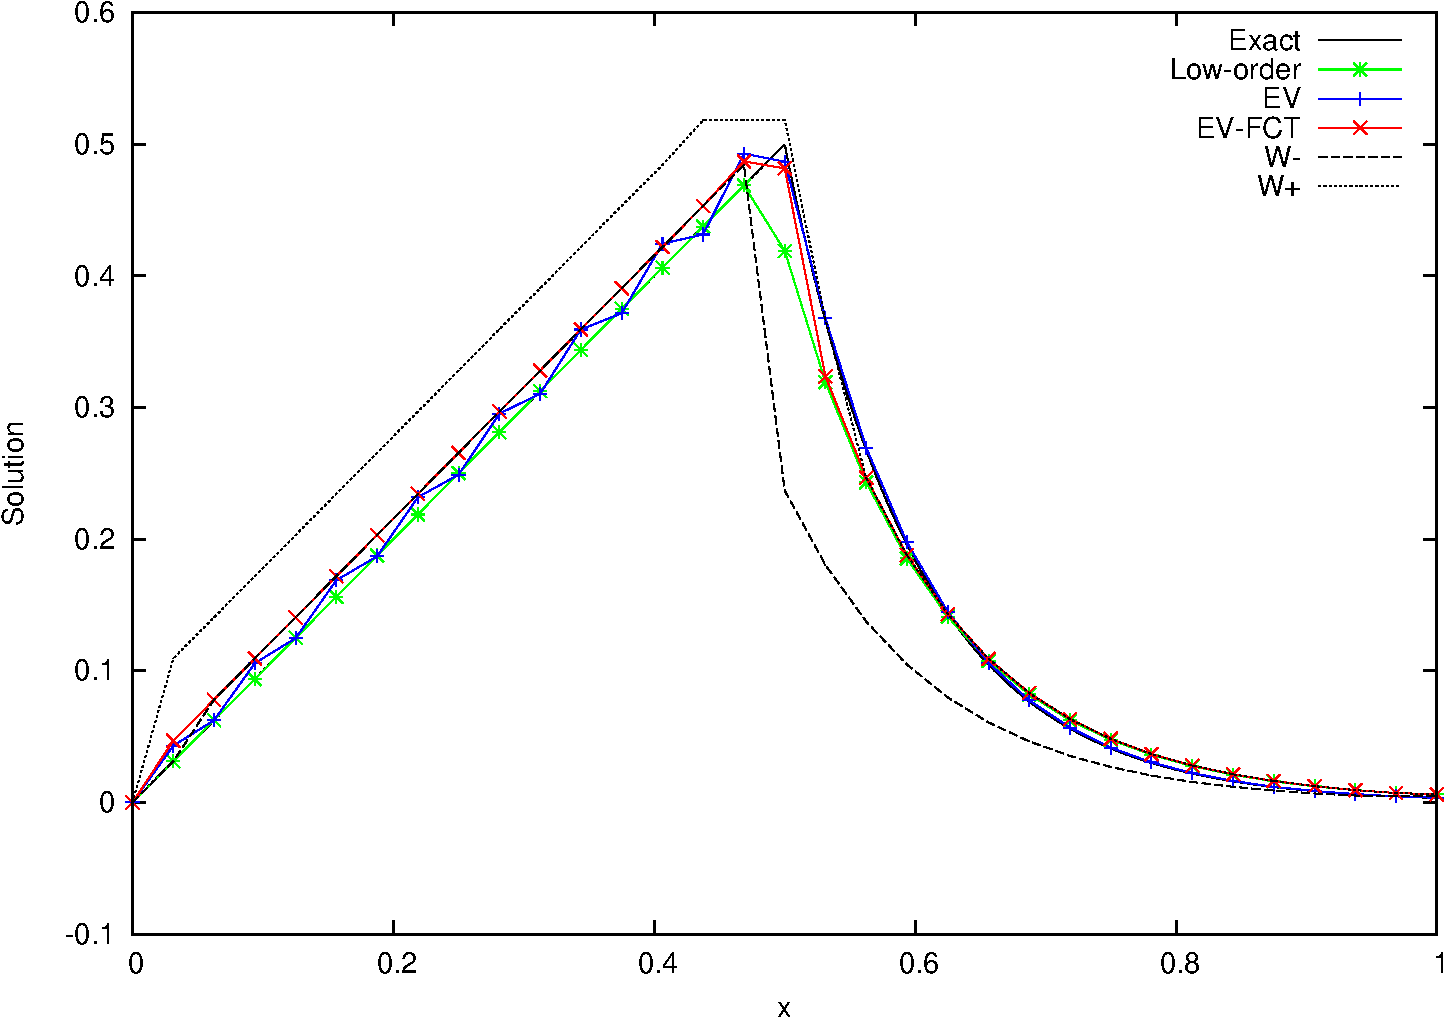
\includegraphics[width=\textwidth]
     {\contentdir/results/transport/source_void_to_absorber/images/weak_with_penalty.pdf}
   \caption{Steady-State Solutions for the Source-Void-to-Absorber Problem
     with Weakly Imposed Dirichlet Boundary Conditions and Boundary Penalty}
   \label{fig:source_void_to_absorber_penalty}
\end{figure}
%-------------------------------------------------------------------------------

Table \ref{tab:source_void_to_absorber_be_iterations_cells} shows the
results of a study of the number of EV and FCT iterations for
BE time discretization, required in
a transient with a constant CFL of 1 and varying mesh sizes. The
results in the table show a decrease in the number of EV iterations
per time step, and a relatively constant number of FCT iterations per
time step.

%-------------------------------------------------------------------------------
\begin{center}
\begin{table}[ht]
\caption{Nonlinear Iterations vs. Number of Cells for the
  Source-Void-to-Absorber Test Problem Using Implicit Euler Time Discretization
  with CFL = 1}
\label{tab:source_void_to_absorber_be_iterations_cells}
\begin{tabular}{c c c c c}\toprule
$N_{cell}$ & \multicolumn{2}{c}{\emph{EV}} & \multicolumn{2}{c}{\emph{FCT}}\\
           & \emph{Total} & \emph{Avg.}    &  \emph{Total} & \emph{Avg.}\\\midrule
  8 &  661 & 24.48 &   244 &  9.04\\
 16 &  807 & 19.21 &   655 & 15.60\\
 32 &  844 & 11.25 &  1194 & 15.92\\
 64 & 1204 &  8.72 &  2024 & 14.67\\
128 & 1752 &  6.59 &  3675 & 13.82\\
256 & 2713 &  5.20 &  6673 & 12.78\\
512 & 4284 &  4.14 & 12098 & 11.69\\
\bottomrule\end{tabular}
\end{table}
\end{center}
%-------------------------------------------------------------------------------

Table \ref{tab:source_void_to_absorber_be_iterations_cfl} shows
the results of a study of nonlinear iterations vs. CFL number for
implicit Euler time discretization and 128 cells. The general
trend shows that entropy viscosity iterations per time step gradually increase
with increasing CFL, while FCT iterations per time step increases
much more quickly. Even more problematic is that the EV-FCT solution
error jumps very quickly from CFLs $\nu=5$ to $\nu=10$.

%-------------------------------------------------------------------------------
\begin{table}[htb]
\caption{Nonlinear Iterations vs. CFL Number for the
 Source-Void-to-Absorber Test Problem Using Implicit Euler Time Discretization
 with 128 Cells}
\label{tab:source_void_to_absorber_be_iterations_cfl}
\centering
\begin{tabular}{c c c c c c c }\toprule
 & & \multicolumn{2}{c}{\emph{EV}}
  & \multicolumn{2}{c}{\emph{FCT}} &\\
\emph{CFL} & $N_{step}$ & \emph{Total} & \emph{Avg.}
  & \emph{Total} & \emph{Avg.} & $L^2$ \emph{err.}\\\midrule
0.1 & 2661 & 15006 &  5.64 & 14036 &   5.27 & $3.013\times10^{-3}$\\
0.5 &  533 &  3445 &  6.46 &  5000 &   9.38 & $3.033\times10^{-3}$\\
1.0 &  266 &  1752 &  6.59 &  3675 &  13.82 & $3.023\times10^{-3}$\\
5.0 &   54 &   471 &  8.72 & 12208 & 226.07 & $2.979\times10^{-3}$\\
10.0 &  27 &   232 &  8.59 &  6126 & 226.89 & $3.325\times10^{-3}$\\
20.0 &  14 &   133 &  9.50 &  3713 & 265.21 & $3.727\times10^{-3}$\\
50.0 &   6 &    62 & 10.33 &  2077 & 346.17 & $7.191\times10^{-3}$\\
\bottomrule\end{tabular}
\end{table}
%-------------------------------------------------------------------------------

\clearpage
